% ============================================================
% Multivariate Statistics — Final Project Report
% YSU Master's Program, 2025/2026
% Compile on Overleaf (pdfLaTeX)
% Upload all plot_*.png files alongside this .tex file
% ============================================================
\documentclass[11pt, a4paper]{article}

\usepackage[top=2cm, bottom=2cm, left=2.2cm, right=2.2cm]{geometry}
\usepackage{amsmath, amssymb}
\usepackage{graphicx}
\usepackage{booktabs}
\usepackage{caption}
\usepackage{subcaption}
\usepackage{float}
\usepackage{hyperref}
\usepackage{setspace}
\usepackage{parskip}
\usepackage{titlesec}
\usepackage{xcolor}
\usepackage{microtype}
\usepackage{listings}
\usepackage{enumitem}
\usepackage{array}
\usepackage{multirow}

% Section formatting — compact
\titleformat{\section}{\large\bfseries}{}{0em}{}[\titlerule]
\titleformat{\subsection}{\normalsize\bfseries}{}{0em}{}
\titlespacing*{\section}{0pt}{10pt}{4pt}
\titlespacing*{\subsection}{0pt}{6pt}{2pt}

\setlength{\parskip}{4pt}
\setlength{\parindent}{0pt}
\captionsetup{font=small, labelfont=bf, skip=4pt}

% Code style for appendix
\lstset{
  language=Python,
  basicstyle=\ttfamily\footnotesize,
  keywordstyle=\color{blue},
  commentstyle=\color{gray},
  stringstyle=\color{orange!80!black},
  breaklines=true,
  frame=single,
  numbers=left, numberstyle=\tiny\color{gray},
  numbersep=5pt,
  showstringspaces=false,
  tabsize=2,
}

\hypersetup{colorlinks=true, linkcolor=black, urlcolor=blue, citecolor=black}

% ============================================================
\begin{document}

\begin{center}
  {\LARGE\bfseries Multivariate Statistical Analysis of\\[4pt]
  WHO Life Expectancy Data}\\[8pt]
  {\large Yerevan State University — Master's Programme in Statistics}\\[4pt]
  {\normalsize Academic Year 2025/2026 \quad|\quad Instructor: A.\ Dalalyan}\\[4pt]
  {\normalsize \textbf{[Name Surname]}}\\[4pt]
  {\small Code repository: \url{https://github.com/[tarkha01]/multivariate-stat}}
\end{center}

\vspace{-4pt}\hrule\vspace{6pt}

% ============================================================
\section{Dataset Description}

The dataset used is the \textbf{WHO Life Expectancy dataset} (2000–2015), 
publicly available on Kaggle.\footnote{%
\url{https://www.kaggle.com/datasets/kumarajarshi/life-expectancy-who}}
After removing rows with missing values, the working dataset contains
\textbf{2{,}311 observations} across \textbf{155 countries} and \textbf{16 years},
with 8 quantitative variables (Table~\ref{tab:vars}).

This dataset is particularly interesting because it links macroeconomic indicators
(GDP, schooling) with health outcomes (life expectancy, child mortality), enabling
us to quantify the relative contribution of economic development versus direct
health factors to population longevity.

\begin{table}[H]
\centering
\caption{Variables and summary statistics ($n = 2{,}311$)}
\label{tab:vars}
\small
\begin{tabular}{llrrrr}
\toprule
\textbf{Variable} & \textbf{Description} & \textbf{Mean} & \textbf{SD} & \textbf{Min} & \textbf{Max}\\
\midrule
\texttt{Life\_expectancy} $\dagger$ & Life expectancy (years) & 69.34 & 9.70 & 36.3 & 89.0\\
\texttt{Adult\_Mortality} & Deaths per 1{,}000 adults (15–60 yrs) & 161.6 & 127.7 & 1.0 & 723.0\\
\texttt{Alcohol} & Per-capita alcohol (litres, pure) & 4.61 & 4.03 & 0.0 & 17.9\\
\texttt{BMI} & Average national BMI & 38.11 & 19.81 & 1.4 & 77.1\\
\texttt{HIVAIDS} & HIV/AIDS deaths per 1{,}000 live births & 1.97 & 5.62 & 0.1 & 50.6\\
\texttt{GDP} & GDP per capita (USD) & 7{,}597 & 14{,}518 & 2 & 119{,}173\\
\texttt{Schooling} & Average years of schooling & 12.10 & 3.35 & 0.0 & 20.7\\
\texttt{Income\_composition} & HDI income index (0–1) & 0.63 & 0.21 & 0.0 & 0.95\\
\bottomrule
\end{tabular}
\vspace{2pt}

{\small $\dagger$ Dependent variable. Developing: 1{,}888 obs.; Developed: 423 obs.}
\end{table}

% ============================================================
\section{Scatter Plot Matrix}

Figure~\ref{fig:scatter} shows three variants of the scatter plot matrix for five
key variables. 

\begin{figure}[H]
  \centering
  \begin{subfigure}[t]{0.32\textwidth}
    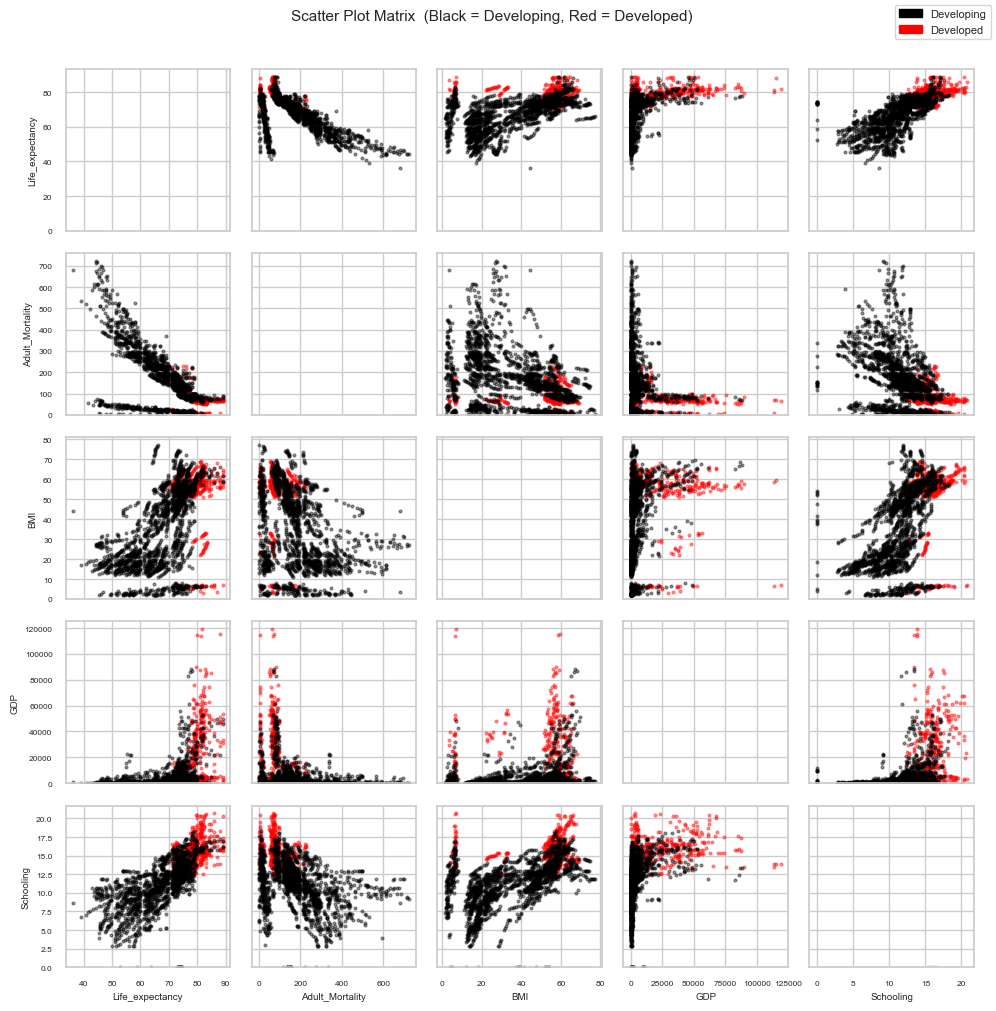
\includegraphics[width=\linewidth]{plot_01_scattermatrix_basic.png}
    \caption{Colored by status}
  \end{subfigure}\hfill
  \begin{subfigure}[t]{0.32\textwidth}
    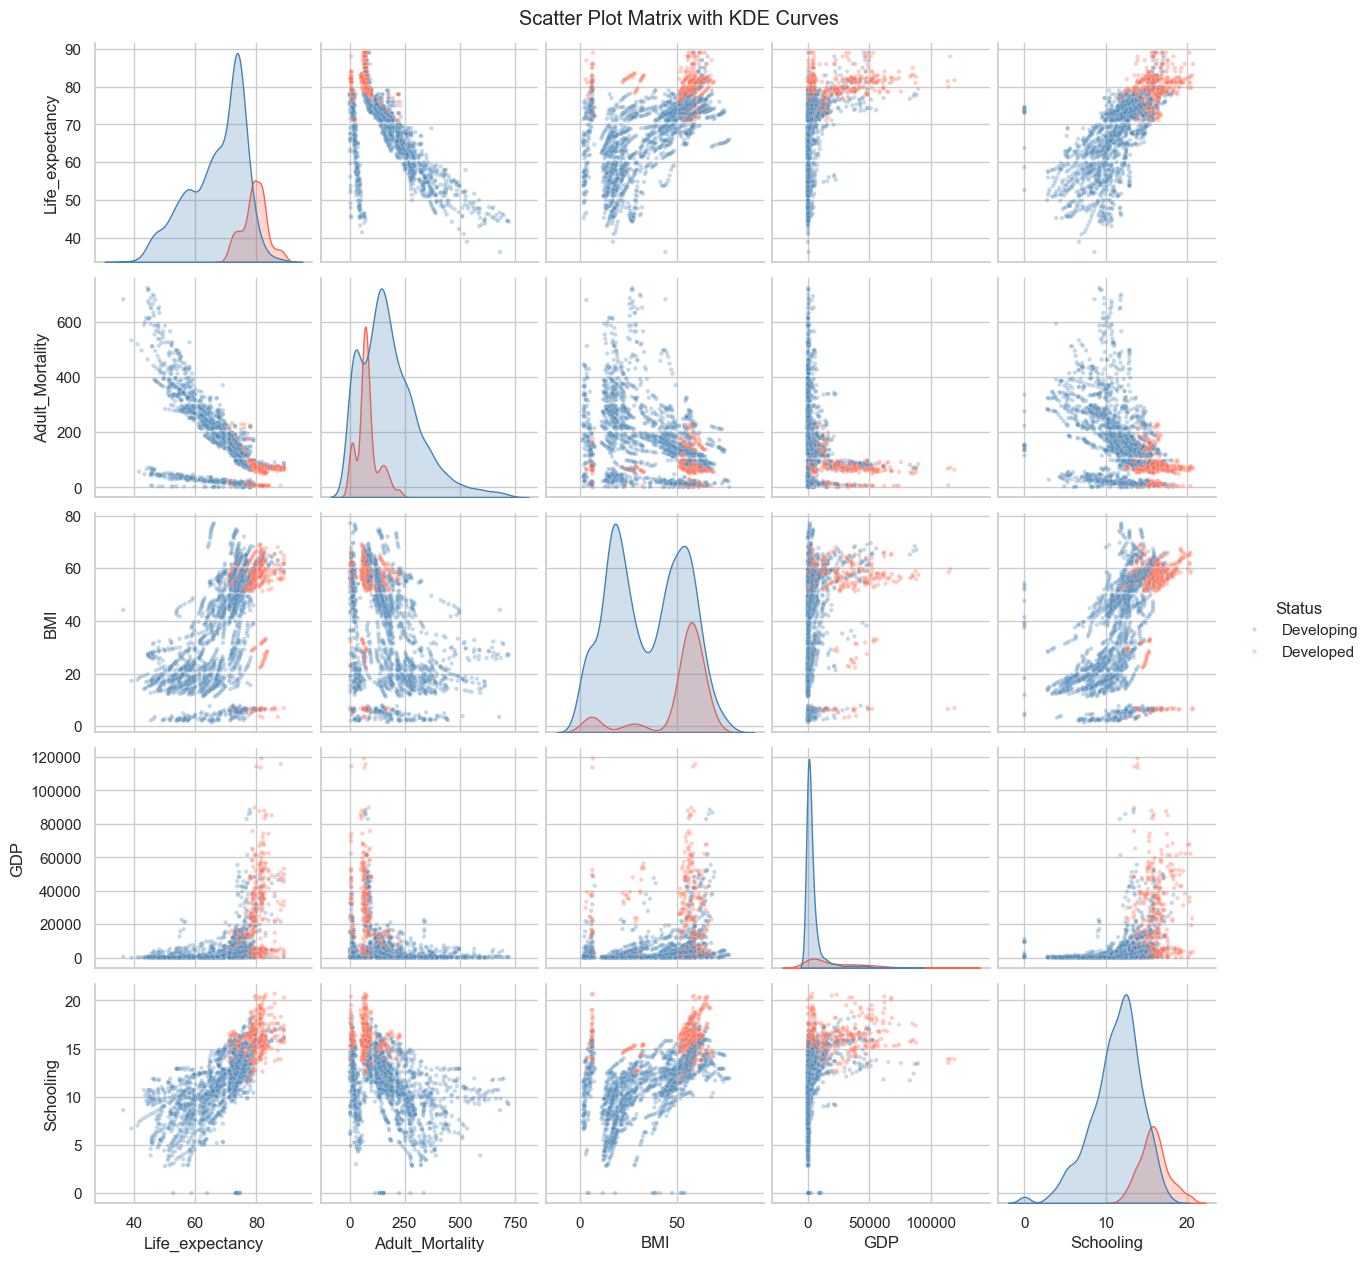
\includegraphics[width=\linewidth]{plot_02_scattermatrix_kde.png}
    \caption{With KDE on diagonal}
  \end{subfigure}\hfill
  \begin{subfigure}[t]{0.32\textwidth}
    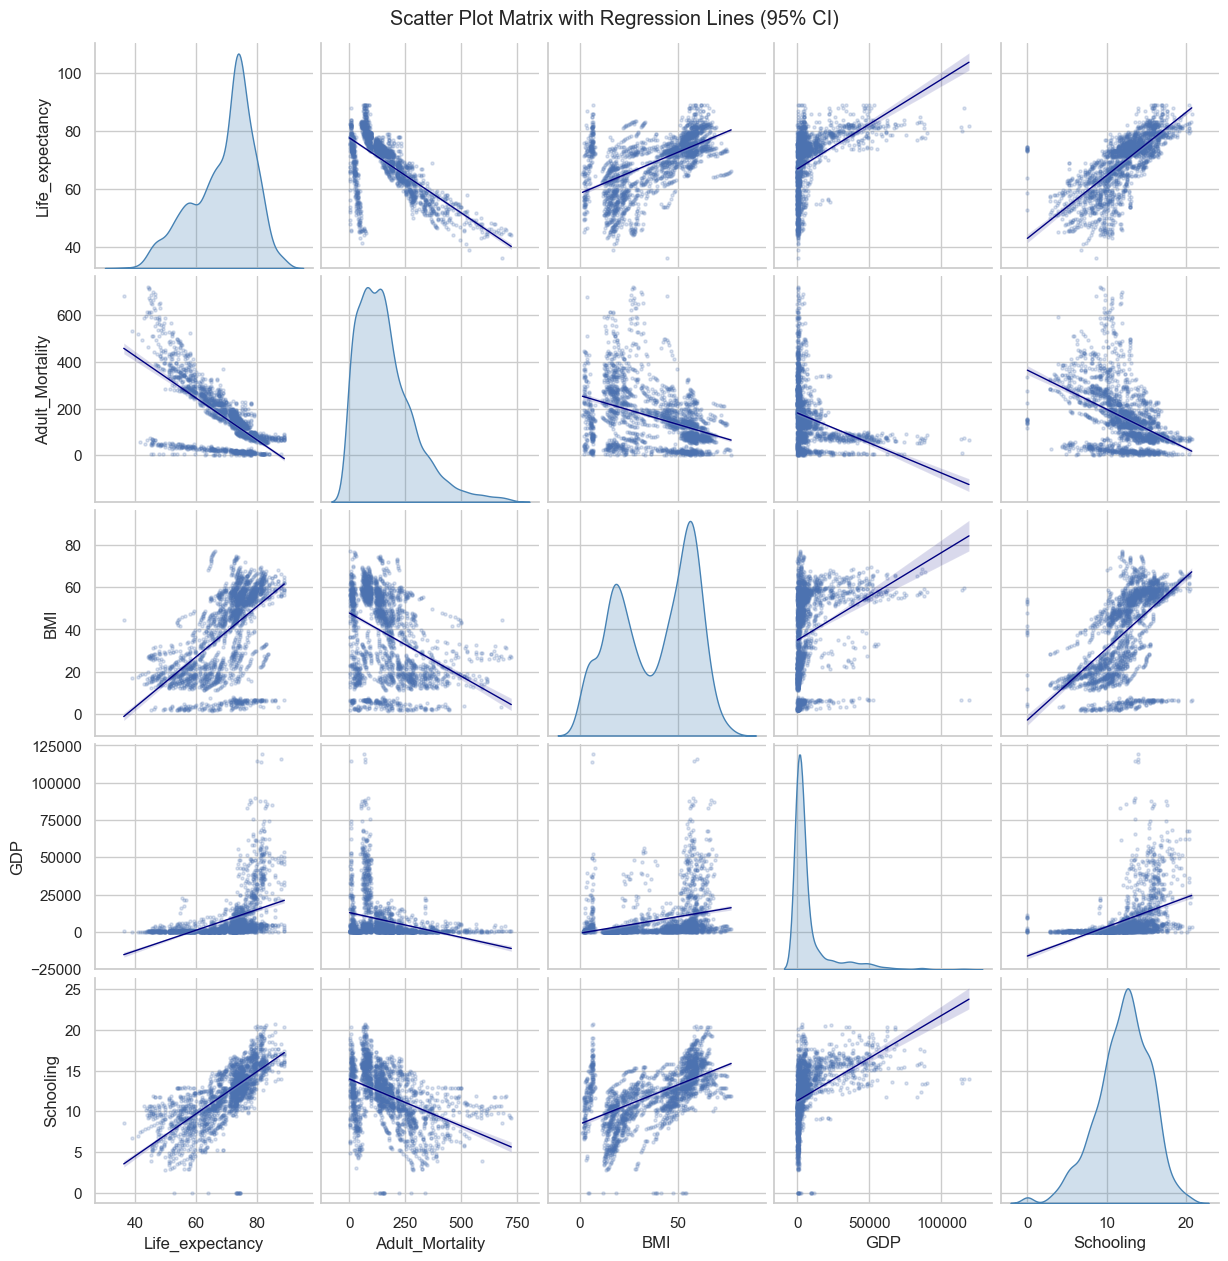
\includegraphics[width=\linewidth]{plot_03_scattermatrix_regression.png}
    \caption{With regression lines}
  \end{subfigure}
  \caption{Scatter plot matrix (black/blue = Developing, red = Developed).}
  \label{fig:scatter}
\end{figure}

Several strong pairwise relationships are visible. \texttt{Life\_expectancy}
decreases sharply with \texttt{Adult\_Mortality} (negative, roughly linear).
It increases with \texttt{Schooling} (positive, nearly linear).
The regression lines in panel~(c) reveal a slight \emph{non-linearity} in the
\texttt{GDP}–\texttt{Life\_expectancy} relationship, suggesting a logarithmic
saturation effect at very high income levels.
Developed countries (red) cluster in the upper-right quadrant — high schooling,
high BMI, low mortality, high life expectancy — while Developing countries (black)
show much greater dispersion, indicating within-group heterogeneity.

% ============================================================
\section{Normality Assessment}

\subsection{Univariate tests}
The Shapiro--Wilk test (Table~\ref{tab:normality}) rejects normality for all eight
variables at any conventional significance level ($p \approx 0$).
The Q-Q plots (Figure~\ref{fig:qq}) confirm heavy right-skew in \texttt{GDP} and
\texttt{HIVAIDS}, a bimodal shape in \texttt{Life\_expectancy}
(separating developed and developing countries), and excess kurtosis throughout.

\begin{table}[H]
\centering
\caption{Shapiro--Wilk normality test results}
\label{tab:normality}
\small
\begin{tabular}{lrrr}
\toprule
\textbf{Variable} & \textbf{W statistic} & \textbf{$p$-value} & \textbf{Normal?}\\
\midrule
Life\_expectancy & 0.9528 & $\approx 0$ & No \\
Adult\_Mortality & 0.9014 & $\approx 0$ & No \\
Alcohol & 0.9128 & $\approx 0$ & No \\
BMI & 0.9250 & $\approx 0$ & No \\
HIVAIDS & 0.3719 & $\approx 0$ & No \\
GDP & 0.5557 & $\approx 0$ & No \\
Schooling & 0.9850 & $\approx 0$ & No \\
Income\_composition & 0.9073 & $\approx 0$ & No \\
\bottomrule
\end{tabular}
\end{table}

\begin{figure}[H]
  \centering
  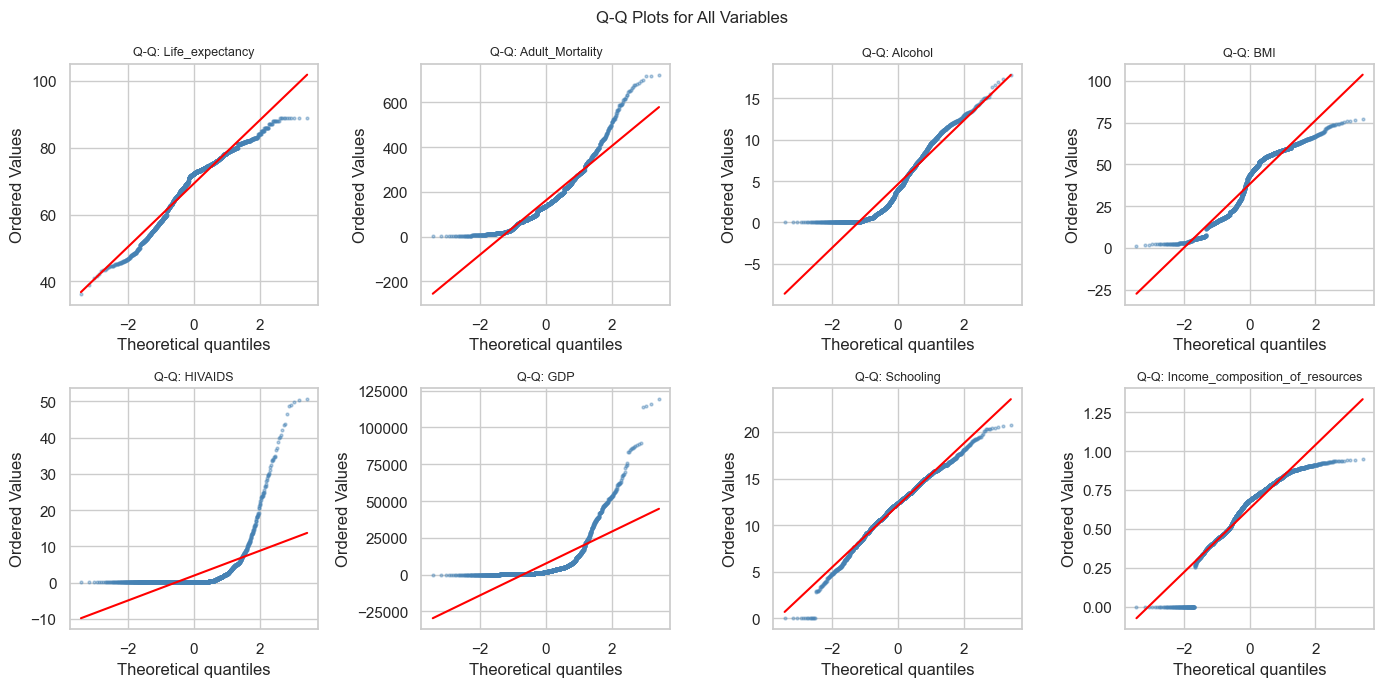
\includegraphics[width=0.9\linewidth]{plot_04_qqplots.png}
  \caption{Q-Q plots. Red line = theoretical normal quantiles.
           Deviations indicate skewness and heavy tails.}
  \label{fig:qq}
\end{figure}

\subsection{Multivariate normality — Mardia's test}
Mardia's test also rejects multivariate normality: 
skewness $\chi^2 = 28{,}227$ ($p \approx 0$),
kurtosis $z = 34{,}949$ ($p \approx 0$).
After log-transforming \texttt{GDP}, \texttt{HIVAIDS}, and \texttt{Adult\_Mortality},
the skewness statistic drops to 32.9, but the data remain significantly non-normal.
\textbf{Conclusion:} the Gaussian assumption is not tenable for this dataset,
which is expected for cross-national health data aggregated over 16 years.
Nevertheless, the OLS regression and PCA procedures below remain
valid approximations under the large-sample regime ($n = 2{,}311$).

% ============================================================
\section{Linear Regression}

\subsection{Model and results}

\texttt{Life\_expectancy} was chosen as the dependent variable because it is the
primary aggregate health outcome that the remaining variables theoretically
influence — it is the ``output'' of the health-development system.

The full OLS model is:
\[
  \widehat{\texttt{LifeExp}} = 53.51
  - 0.017\,\texttt{AdultMort}
  - 0.028\,\texttt{Alcohol}
  + 0.053\,\texttt{BMI}
  - 0.499\,\texttt{HIV}
  + 0.00006\,\texttt{GDP}
  + 0.987\,\texttt{Schooling}
  + 8.457\,\texttt{Income}
\]

\begin{table}[H]
\centering
\caption{OLS regression results. $R^2 = 0.811$, Adj.\ $R^2 = 0.810$, $F(7{,}2303) = 1412$, $p<0.001$.}
\label{tab:ols}
\small
\begin{tabular}{lrrrrl}
\toprule
\textbf{Variable} & \textbf{Coef.} & \textbf{Std.\ Err.} & \textbf{$t$} & \textbf{$p$-value} & \textbf{VIF}\\
\midrule
Intercept & 53.513 & 0.461 & 116.14 & $<$0.001 & —\\
Adult\_Mortality & $-$0.017 & 0.001 & $-$18.96 & $<$0.001 & 1.74\\
Alcohol & $-$0.028 & 0.027 & $-$1.04 & 0.299 & 1.51\\
BMI & 0.053 & 0.006 & 9.53 & $<$0.001 & 1.56\\
HIVAIDS & $-$0.499 & 0.019 & $-$26.61 & $<$0.001 & 1.43\\
GDP & $5.8\times10^{-5}$ & $7.0\times10^{-6}$ & 8.25 & $<$0.001 & 1.34\\
Schooling & 0.987 & 0.049 & 20.19 & $<$0.001 & 3.47\\
Income\_composition & 8.457 & 0.704 & 12.02 & $<$0.001 & 2.96\\
\bottomrule
\end{tabular}
\end{table}

The model explains \textbf{81.1\%} of variance in life expectancy.
All predictors except \texttt{Alcohol} are highly significant ($p < 0.001$).
The strongest positive effect comes from \texttt{Income\_composition} (+8.46 years
per unit increase in the HDI income index) and \texttt{Schooling} (+0.99 years per
additional year of schooling). The strongest negative effect is from \texttt{HIVAIDS}
($-0.50$ years per unit increase in child HIV mortality).
All VIF values are below~5, indicating no multicollinearity problem.

% ============================================================
\section{Variable Selection}

Three methods were applied to identify the most informative predictors.
All three consistently \textbf{exclude \texttt{Alcohol}} and retain the remaining six variables.

\begin{table}[H]
\centering
\caption{Variable selection — model comparison}
\label{tab:varsel}
\small
\begin{tabular}{lrrrr}
\toprule
\textbf{Method} & \textbf{$R^2$} & \textbf{Adj.\ $R^2$} & \textbf{AIC} & \textbf{\# Vars}\\
\midrule
Full model (7 vars) & 0.8110 & 0.8104 & 13{,}227.4 & 7\\
Stepwise AIC & 0.8109 & 0.8104 & 13{,}226.5 & 6\\
LASSO ($\lambda^* = 0.137$) & 0.8109 & 0.8104 & 13{,}226.5 & 6\\
\bottomrule
\end{tabular}
\end{table}

The forward subset selection shows that \texttt{Schooling} alone explains 56.3\%
of variance; adding \texttt{HIVAIDS} raises it to 73.5\%, and including
\texttt{Adult\_Mortality} and \texttt{Income\_composition} brings it to 79.7\%.
The last marginal gain comes from adding \texttt{GDP} (6th variable, Adj.\ $R^2 = 0.8104$).
\textbf{Interpretation:} \texttt{Alcohol} is redundant — its effect is already captured by the
socioeconomic variables, and its regression coefficient is not significantly different from zero.

% ============================================================
\section{Principal Component Analysis}

\subsection{Eigenvalues and explained variance}

PCA was performed on standardised data. Table~\ref{tab:pca} shows the eigenvalue
decomposition. The Kaiser criterion (eigenvalue $> 1$) retains \textbf{PC1 and PC2},
which together explain \textbf{68.4\%} of total variance.

\begin{table}[H]
\centering
\caption{PCA eigenvalues and variance explained}
\label{tab:pca}
\small
\begin{tabular}{lrrr}
\toprule
\textbf{PC} & \textbf{Eigenvalue} & \textbf{Variance (\%)} & \textbf{Cumulative (\%)}\\
\midrule
PC1 & 4.191 & 52.36 & 52.36\\
PC2 & 1.279 & 15.99 & 68.35\\
PC3 & 0.704 & 8.80 & 77.15\\
PC4 & 0.588 & 7.35 & 84.50\\
PC5–PC8 & — & 15.50 & 100.00\\
\bottomrule
\end{tabular}
\end{table}

\textbf{PC1} (52.4\%) is a \emph{health-development axis}: high positive loadings for
\texttt{Life\_expectancy} (0.447), \texttt{Schooling} (0.423), and
\texttt{Income\_composition} (0.412), opposed by negative loadings for
\texttt{Adult\_Mortality} ($-0.337$) and \texttt{HIVAIDS} ($-0.244$).
Countries scoring high on PC1 have long lives, good education, and low mortality.
\textbf{PC2} (16.0\%) separates countries by \emph{disease burden vs.\ alcohol/BMI
profile}: dominated by \texttt{HIVAIDS} (0.642), \texttt{Alcohol} (0.475), and
\texttt{Adult\_Mortality} (0.438).

\begin{figure}[H]
  \centering
  \begin{subfigure}[t]{0.46\textwidth}
    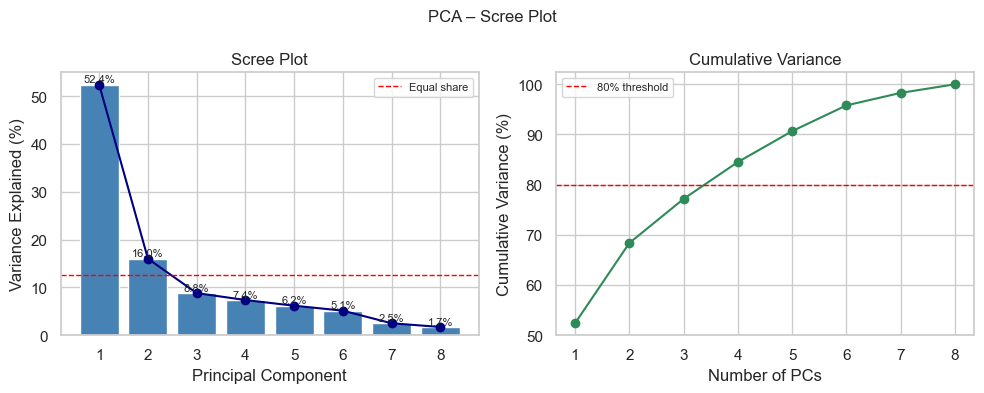
\includegraphics[width=\linewidth]{plot_09_screeplot.png}
    \caption{Scree plot}
  \end{subfigure}\hfill
  \begin{subfigure}[t]{0.50\textwidth}
    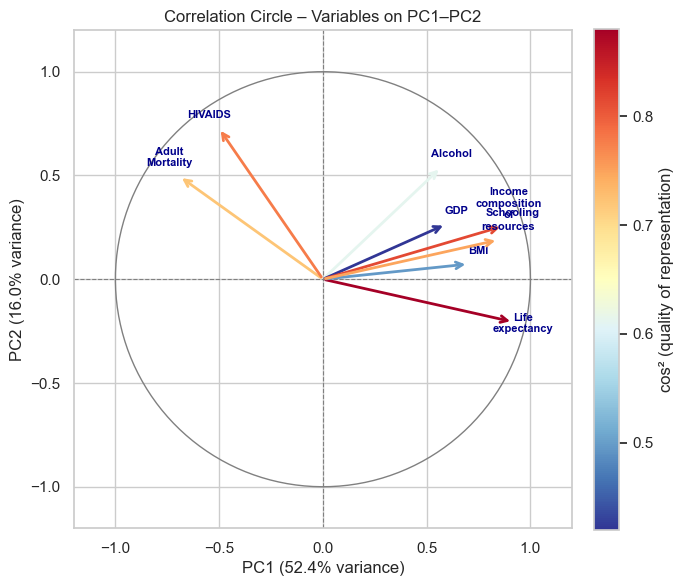
\includegraphics[width=\linewidth]{plot_10_correlation_circle.png}
    \caption{Correlation circle}
  \end{subfigure}
  \caption{PCA visualisations. Left: variance explained per component.
           Right: variables on the PC1–PC2 plane, coloured by cos$^2$ (quality of representation).}
  \label{fig:pca}
\end{figure}

% ============================================================
\section{Correlation Circle}

The correlation circle (Figure~\ref{fig:pca}b) reveals the structure of
inter-variable relationships projected onto the first two principal components.

\begin{itemize}[noitemsep, topsep=2pt]
  \item \texttt{Life\_expectancy}, \texttt{Schooling}, and \texttt{Income\_composition}
        point in the same direction (positive PC1), forming a \emph{socio-health cluster}.
        Their near-parallel arrows indicate strong pairwise positive correlations
        (confirmed: $r_{\text{Schooling, Income}} = 0.797$).
  \item \texttt{Adult\_Mortality} and \texttt{HIVAIDS} point in the opposite direction
        (negative PC1), anti-correlated with the socio-health cluster.
  \item \texttt{Alcohol} has a large PC2 component, meaning it is \emph{orthogonal}
        to the health-development axis — it provides distinct information not captured by PC1,
        consistent with its non-significance in the regression model.
  \item \texttt{GDP} has moderate length on both axes, indicating partial, but not perfect,
        representation in this 2D projection.
\end{itemize}

% ============================================================
\section{Individual Projections onto PC1--PC2}

\begin{figure}[H]
  \centering
  \begin{subfigure}[t]{0.50\textwidth}
    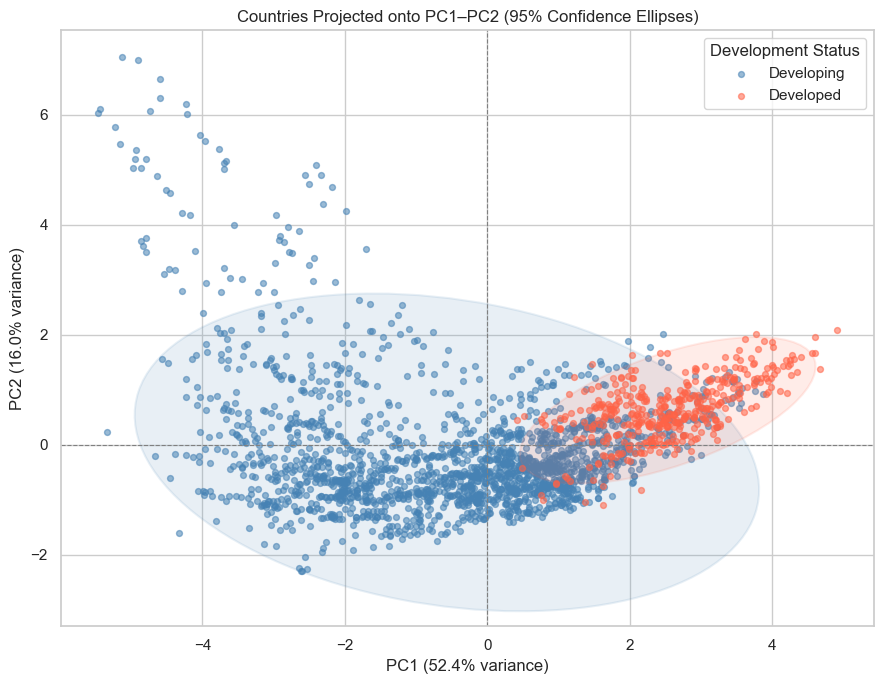
\includegraphics[width=\linewidth]{plot_11_pca_individuals.png}
    \caption{Colored by development status}
  \end{subfigure}\hfill
  \begin{subfigure}[t]{0.46\textwidth}
    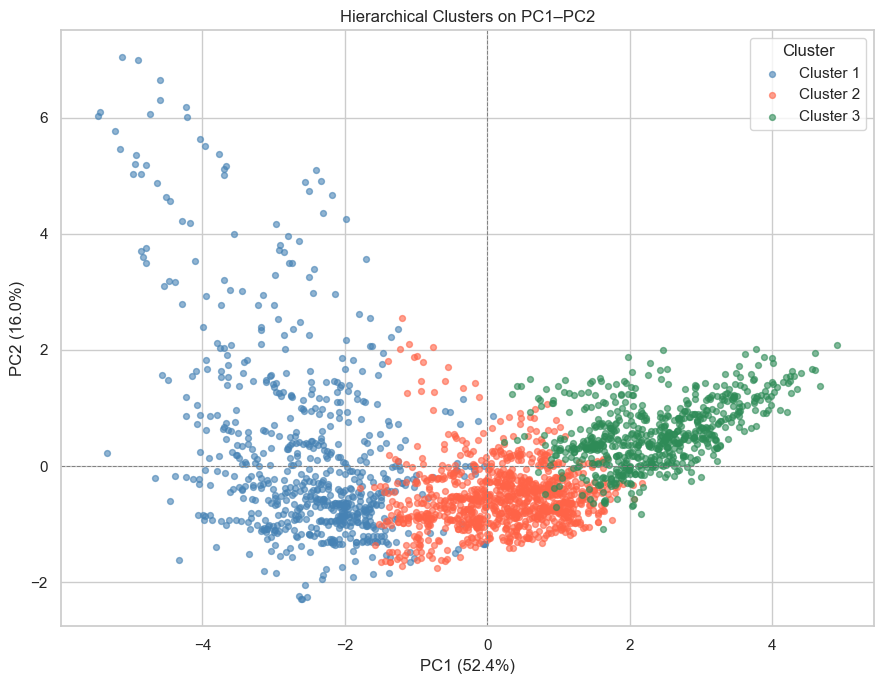
\includegraphics[width=\linewidth]{plot_15_clusters_pca.png}
    \caption{Hierarchical clusters ($k=3$)}
  \end{subfigure}
  \caption{Projection of country-year observations onto PC1–PC2.}
  \label{fig:indiv}
\end{figure}

\textbf{Developed} countries (tomato ellipse) form a tight, compact cluster in the
positive PC1 region, confirming homogeneous health-development profiles.
\textbf{Developing} countries (blue ellipse) are widely scattered along both axes,
reflecting the enormous heterogeneity of the developing world — from rapidly-improving
Asian economies to high-HIV-burden Sub-Saharan African countries.
The hierarchical clustering ($k=3$, Ward's linkage) provides a finer separation:
\emph{Cluster 1} (low-income, $\bar{y}=57.7$ yrs, high HIV/AIDS)
corresponds to Sub-Saharan Africa;
\emph{Cluster 2} (middle-income, $\bar{y}=71.7$ yrs) to the bulk of developing nations;
\emph{Cluster 3} (high-income, $\bar{y}=78.3$ yrs, GDP$\approx$\$20{,}888)
to developed and upper-middle-income countries.

% ============================================================
\section*{Conclusions}

This analysis of WHO Life Expectancy data (2311 obs., 155 countries, 2000–2015)
yields five main findings:
\begin{enumerate}[noitemsep, topsep=2pt, label=\arabic*.]
  \item The data are significantly non-Gaussian, driven by cross-national inequality and outliers.
  \item A linear model with 6 variables explains 81.1\% of variance in life expectancy;
        \texttt{Schooling}, \texttt{Income\_composition}, and \texttt{HIVAIDS} are the dominant drivers.
  \item All three variable-selection methods agree: \texttt{Alcohol} is the only redundant predictor.
  \item PCA identifies a dominant ``health-development'' axis (PC1, 52.4\%) that
        separates wealthy/educated nations from high-mortality ones.
  \item Three country clusters emerge, broadly corresponding to low-, middle-, and high-income groups,
        with the largest gap in life expectancy between clusters 1 and 3 ($\approx 20$ years).
\end{enumerate}

% ============================================================
\newpage
\appendix
\section*{Appendix A — Python Code}
\addcontentsline{toc}{section}{Appendix A: Python Code}

Full code is available at:
\url{https://github.com/[your-username]/multivariate-stat/blob/main/analysis.py}

% Code is available at the repository link above.
% To include the code inline, upload analysis.py to Overleaf
% and uncomment the line below:
% \lstinputlisting{analysis.py}

\end{document}
